\glsresetall
\chapter{Results, Analysis and Limitations}
\label{chap:results_analysis_and_limitations}

In this Chapter we present the final results gathered from the ``Data Analysis'' component presented in Chapter~\ref{chap:proposed_solution}~-~\nameref{chap:proposed_solution}, to answer the questions defined in Section~\ref{sec:research_questions}. Results for both questions, ``1. Is there any anomalous service?'' and ``2. How can we measure the quality of tracing?'', are presented as well as a brief discussion regarding both results in Sections~\ref{sec:anomaly_detection} and~\ref{sec:trace_quality_analysis} respectively. Later, in the end of this Chapter, in Section~\ref{sec:limitations_of_opentracing_data}, we explore some limitations regarding the \emph{OpenTracing} data.

\section{Anomaly Detection}
\label{sec:anomaly_detection}

For the first question, the approach was to use the \gls{otp} tool to extract metrics from tracing data to further analyse it using the unsupervised learning algorithm. The implemented algorithm used for metrics extraction is presented in Algorithm~\ref{alg:metrics_extraction_from_tracing}.

After extract metrics, a tool for metrics visualisation (e.g., Grafana) was used to visualise metrics from \emph{OpenTSDB} database. Samples from these visualizations were presented in Figures~\ref{fig:service_calls_samples},~\ref{fig:service_dependency_variation},~\ref{fig:service_avg_response_time_samples} and~\ref{fig:service_status_code_ratio_samples}. Therefore, the method explained in Algorithm~\ref{alg:anomaly_detection} was applied to metrics extracted from tracing data. From this algorithm, a \gls{csv} file is generated containing candidates to ``possible anomalous regions'' for each service presented in the system. Figure~\ref{fig:service_isolation_forest_detections} shows a sample of the result of outliers identified in time-series data for a given hypothetical service.

%\todo{ADD MORE INFO???}

%\vspace{1.0cm}

\begin{figure}
  %\centering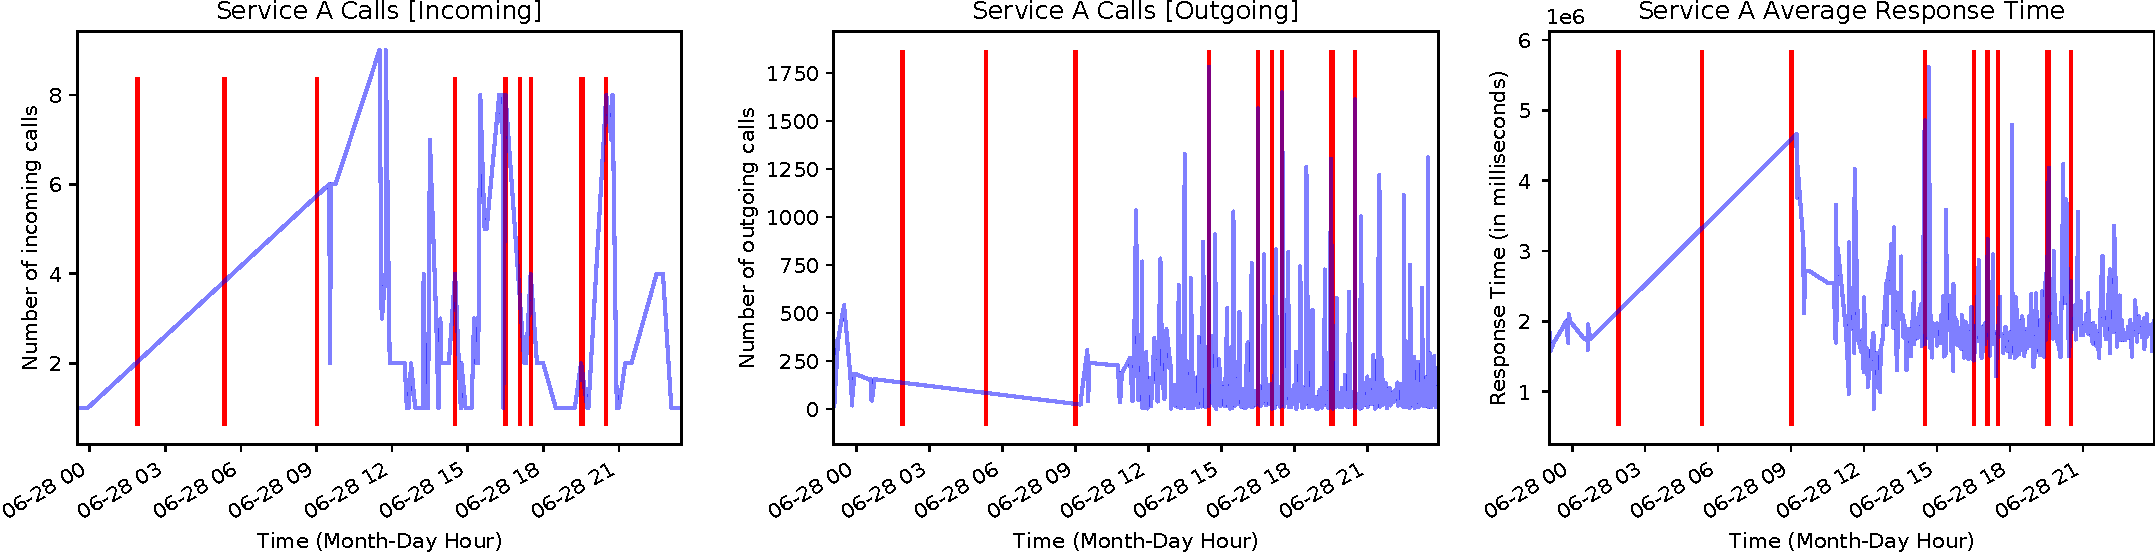
\includegraphics[width=1.0\linewidth]{images/service_isolation_forest_detections.pdf}
  \centering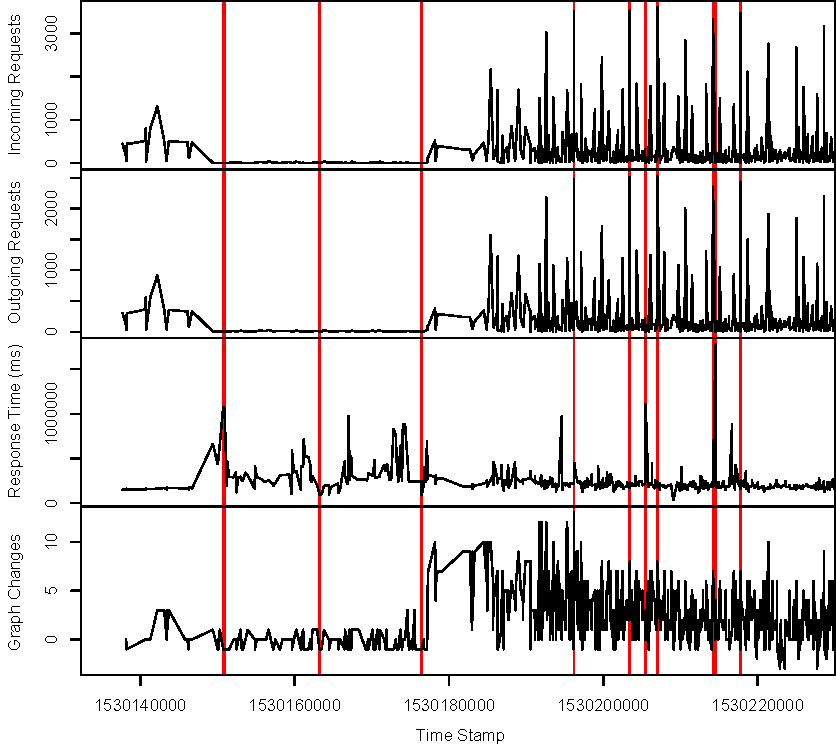
\includegraphics[width=1.0\linewidth]{images/multi_feature_anomaly_detection.pdf}
  \captionsetup{justification=centering}
  \caption{Sample of detection, using multiple feature, of ``Anomalous'' and ``Non-Anomalous'' time-frame regions for a service.}
  \label{fig:service_isolation_forest_detections}
\end{figure}

\newpage

Figure~\ref{fig:service_isolation_forest_detections} contains a set of vertical red lines representing the points of identified anomalies in time, involving the three distinct time-series metrics. From this outlier detection, using \emph{Isolation Forests}, plots containing candidates to ``possible anomalous regions'' were generated. The outcome expected from these plots, were a clustering of values in normal (``non-anomalous'') time-frame regions against clustering of values with outliers scattered in distant regions (``anomalous'').

Figure~\ref{fig:comparison_anomalous_non_anomalous_regions} provides a representation of two time-frame samples, one for the ``anomalous'' region, and the other for the ``non-anomalous'' region considering the same service. In these samples we retrieved data to analyse and give answers to the first question. For this, we considered three features (as shown in the samples bellow): the number of incoming requests, the number of outgoing requests and the average response time. The sample resolution for the time-frame is 10 minutes centred in a given \emph{timestamp}.

\begin{figure}[H]
  \centering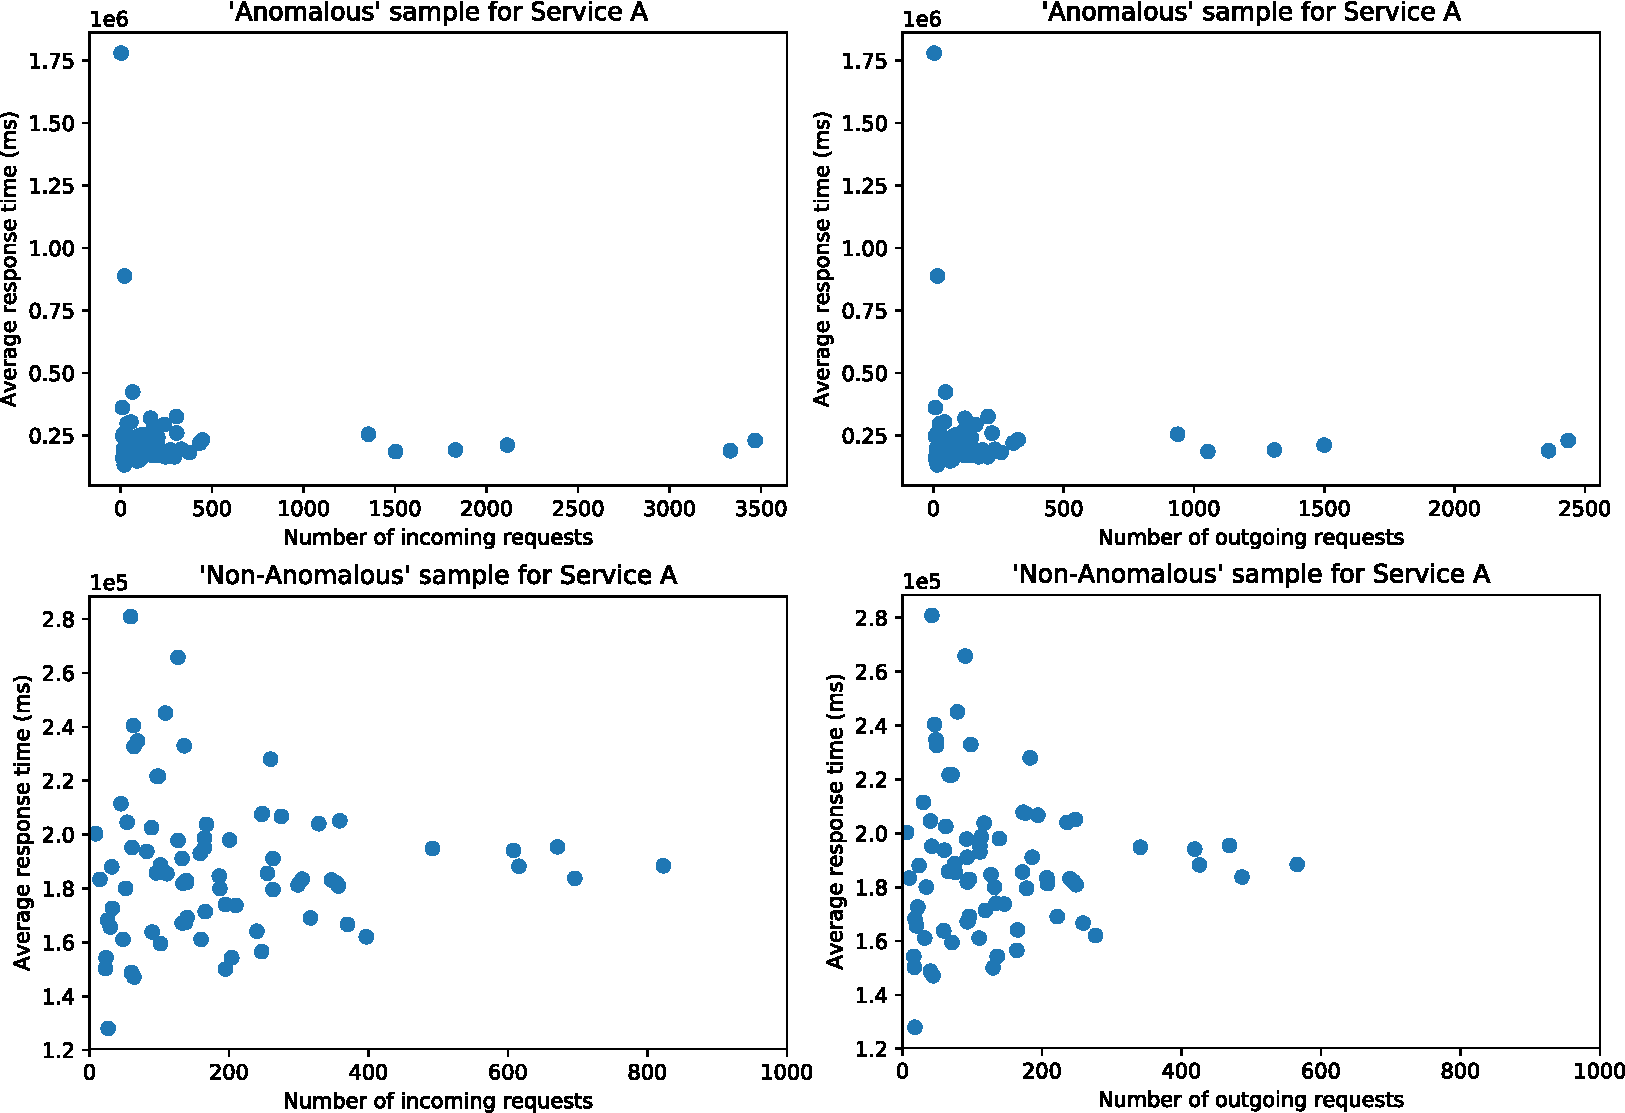
\includegraphics[width=1.0\linewidth]{images/result_samples_for_service_a_cc.pdf}
  \captionsetup{justification=centering}
  \caption{Comparison between ``Anomalous'' and ``Non-Anomalous'' service time-frame regions.}
  \label{fig:comparison_anomalous_non_anomalous_regions}
\end{figure}

As we can see in Figure~\ref{fig:comparison_anomalous_non_anomalous_regions}, there is a clear difference between anomalous and non-anomalous regions. There is a drastic change in the range of values between the anomalous and non-anomalous regions, where the maximum for each feature changes greatly and therefore, outliers are visible and evident in the observations. In the anomalous samples, it is possible to notice a clear crowding of points near the origin point of the chart and some outliers in the upper-left and down-right regions of the chart. On the other side, in the non-anomalous samples, all that is possible to notice is the crowding of points near the origin point of the chart. The crowding of points is what is expected to be the normal behaviour for services, which means that is expected that the service can handle the load with good response times. Furthermore, after this observations, what is expected is to investigate what these points represent and what is causing this unexpected increment in the number of incoming/outgoing requests and the average response time.

There are two anomalous situations observed:

\begin{enumerate}
  \item Services are increasing the response time when there are few incoming/outgoing requests.
  \item Services are receiving more incoming/outgoing requests, however it is having a good response time.
\end{enumerate}

The first situation is much worse than the second one. The expectation is that services can handle more requests and keep the average response time, however, this system is being used for testing purposes, and it has been target of several load and fault injection tests. Furthermore, we do not have access to information regarding this tests, thus we can not be certain if the detected outliers can be considered real ``anomalies'' presented in services, however, they are interesting points to care about due to their unusual values. The worst case scenario would be to find points in the upper-right section of the charts, however this was not observed in this tracing data which leads to the assumption that this system is able to scale their workload well and therefore, it is capable of keeping response time low with large amounts of requests.

To study both situations, and further our anomaly detection presented in services, an analysis of trace request work-flow types was performed. The objective of this analysis is to perceive if there is some strange occurrences in request work-flow paths. To be able to perform this process, the \gls{otp} must be able to get the tracing data and map each unique trace work-flow for the given time-frame. We have used the method presented in Algorithm~\ref{alg:work_flow_type_algorithm} to retrieve this information.

% Removed {alg:work_flow_type_algorithm}

As presented in algorithm~\ref{alg:work_flow_type_algorithm}, parameters from TraceInfo are written to \gls{csv} files. These files are then processed in the ``Data Analyser'' component and, afterwards, a grouping of work-flow types from ``Anomalous'' and ``Non-Anomalous'' regions are retrieved for plotting. Results from this method are presented in Figure~\ref{fig:work_flow_type_analysis}.

\begin{figure}[H]
  \centerline{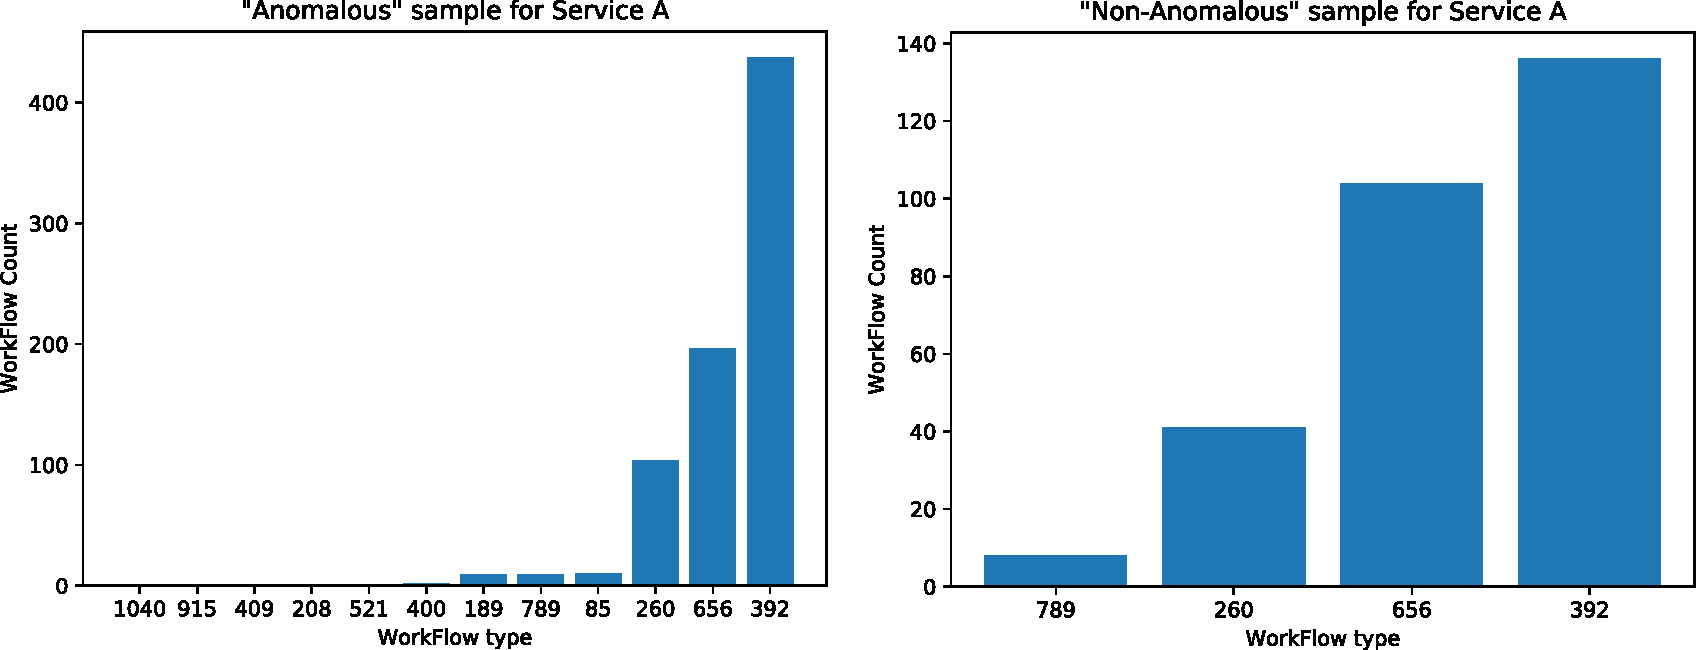
\includegraphics[width=1.0\linewidth]{images/workflow_type_count.pdf}}
  \captionsetup{justification=centering}
  \caption{Comparison between ``Anomalous'' and ``Non-Anomalous'' service work-flow types.}
  \label{fig:work_flow_type_analysis}
\end{figure}

Figure~\ref{alg:work_flow_type_algorithm} shows a clear difference between work-flow types presented in ``anomalous'' and ``non-anomalous'' regions. One interesting thing to notice and that gives more evidence to prove anomalies presented in these regions is that, in the anomalous regions, more quantity and more types of request work-flow types were observed. The next step was to check what was causing this by retrieving the most ``called'' work-flows, however, the results were not good because of the completeness of the tracing data. The flows were not relevant to further our analysis because they were just calls from point A to point B, or represented a not so interesting request path due to involved services. Also, in some of these requests work-flow path, high values of response time were observed and therefore, they tocked longer to execute, however, like for the previous explanation, their path was not relevant to study. For these reasons, there were no possibility to extend our analysis and identify the root cause for these abnormal observed behaviours. Therefore, at this point and for this question, it is possible to say that this data set was exhaustively analysed, and an improvement of the tracing data, or the gathering of other types of data, e.g., monitoring and logging, should be a path to take. One point to note for future work is to test this method with other tracing data, to evaluate them and understand if this approach can lead to identification of the root cause of anomalous behaviour presented in services. For this reason, the data provided and thus, the OpenTracing in general has some limitations. These limitations are covered and explained further in Section~\ref{sec:limitations_of_opentracing_data}.

\section{Trace Quality Analysis}
\label{sec:trace_quality_analysis}

For the second question, the main approach was the same as in for the previous question, we need to use the \gls{otp} to process the tracing data and gather the results to be further analysed in the ``Data Analysis'' component. However, in this case, the results obtained by the first component were directly used by the second one.

In this question the analysis is divided in two procedures as explained in Chapter~\ref{chap:proposed_solution}. The first procedure aims to check if the spans comply with the OpenTracing specification. This method is rather simple and is presented in Algorithm~\ref{alg:span_structure_analysis_algorithm}.

% Removed {alg:span_structure_analysis_algorithm}

The results obtained by the application of this method were that every span structure complies with the specification. This is not a very good test because the specification of the \emph{OpenTracing} is not very strict and therefore, the created method for testing does not provide a very accurate kind of results. To better explain this topic, we give two examples with some solutions for each one. First example, the units for timestamps are not uniform, one can use milliseconds and in other field of a span presented in the same trace, other can use microseconds. This leads to problems in time measurements and is not covered by this test. The solution for this problem can be the standardization of values and use only one measurement unit. Second example, there are multiple declarations for fields with key $\rightarrow$ value pairs, and thus, this brings inconsistency and uncertainty with the possible values that can appear. One solution for this is to redefine the semantic specification and terminology for programmers to adopt in their implementations. The limitations of this specifications and the redefinition of the \emph{OpenTracing} specification is discussed later in Section~\ref{chap:results_analysis_and_limitations}.

% The redefinition of the specification is discussed in Chapter~\ref{chap:conclusion_and_future_work}.

% \todo{Check bellow because it was explained in Ch.6.}

The second procedure aims to check if tracing covers the entire time of the root spans. For a simple example, if we have a trace with a root span of 100 milliseconds of duration, and this root span has two children spans, one with $50ms$, the other one with $10ms$, the entire trace has a coverage of $(50+10)/100=60\%$. This method is applied to every trace, and the results are plotted for visualisation. In this case we apply it and split the results by service, with the objective of perceive the time coverability of tracing in each service. The method is presented in Algorithm~\ref{alg:trace_coverability_analysis} and the corresponding results, regarding two different services, are presented in Figure~\ref{fig:services_coverability_analysis}.

% Removed {alg:trace_coverability_analysis}

\begin{figure}[H]
  \centering{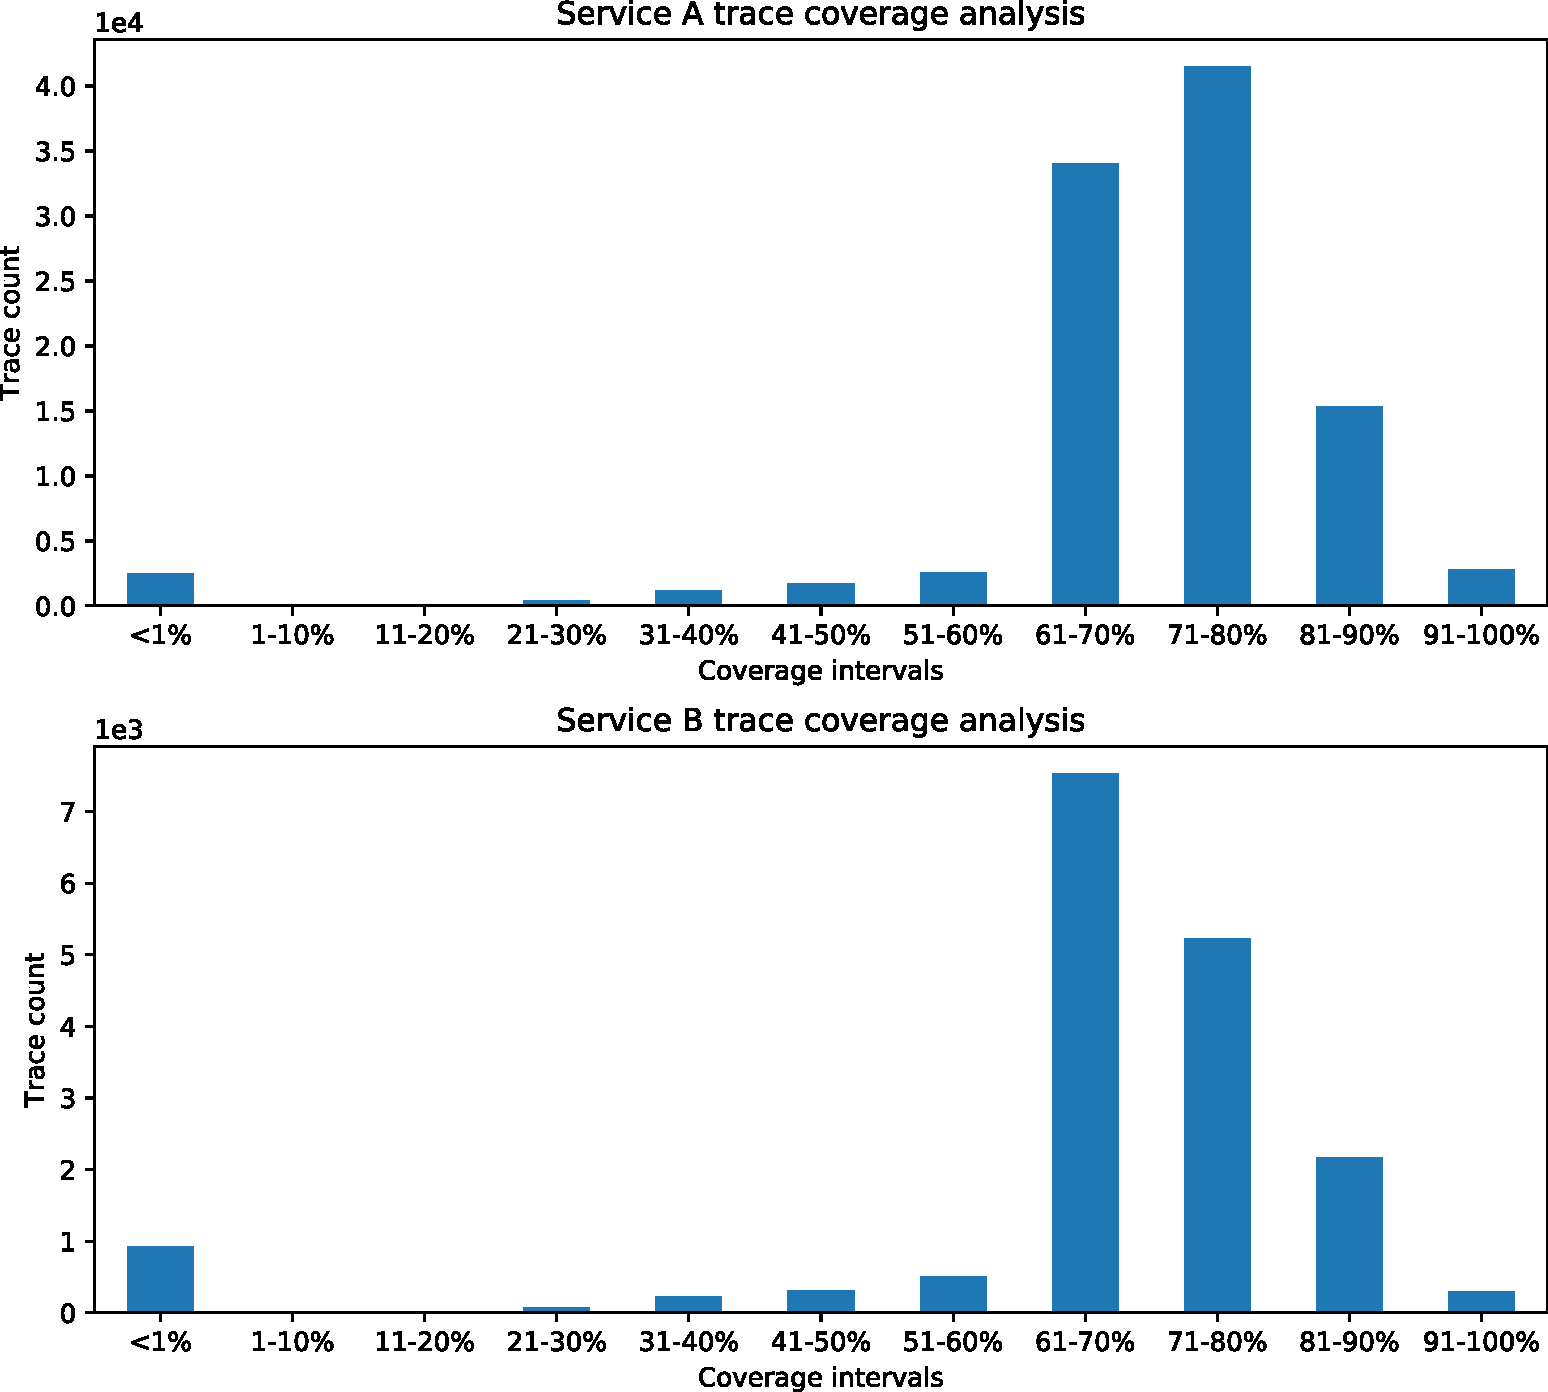
\includegraphics[width=1.0\linewidth]{images/service_trace_coverability_analysis.pdf}}
  \caption{Services coverability analysis.}
  \label{fig:services_coverability_analysis}
\end{figure}

Figure~\ref{fig:services_coverability_analysis} allows the user to visualise the tracing coverability, in terms of how many the overall tracing covers their entire execution duration. The most important thing to notice for this tracing data is the presence of higher bar values in $60\%-100\%$ regions. This means that coverability for this tracing could be better, but in overall is good. What is expected by the result of this kind of analysis is that the coverability of tracing remains closer to the last interval $(90\%-100\%)$, which means that our service is fully/almost fully covered by this kind of data and therefore, the analysis of this data is worthy and the results provided by the usage of this it are trusty. From this data set, the results for the remaining services where close to the ones presented and shown by Figure~\ref{fig:services_coverability_analysis}.

After checking these results, one can use them to see which services developers can analyse in order to improve the coverage of tracing. To improve this coverage, changes in code instrumentation must be performed. Later on, after performing changes in code instrumentation and gather new trace information, the method for coverability test must be executed over the new tracing data to see if results have changed. What is expected is that trace coverability raises, which means that, for example, for service B presented in this figure, after developers changed the implementation, the trace counting for coverage must shift into higher intervals, and for this reason, one must observe lower values for $1\%-70\%$ and higher values for $71\%-100\%$. From this analysis, one thing to improve is to develop a method to analyse the gathered results in order to detect traces that do not cover their duration with respect to a predefined threshold. For example, the method could be applied to newer services after some time (to gather sufficient trace information), and then report or notify the developer if the service does not comply with the predefined coverage threshold. This would allow developers to improve their tracing coverage.

\section{Limitations of OpenTracing Data}
\label{sec:limitations_of_opentracing_data}

In this Section, we explore limitations felted when using and only using \emph{OpenTracing} data in this research and therefore, give some solutions to improve this work and present a brand new project that emerged in the end of this research.

Limitations of \emph{OpenTracing} were exposed in previous topics, Sections~\ref{sec:anomaly_detection} and ~\ref{sec:trace_quality_analysis}. These limitations are presented bellow:

\begin{enumerate}
  \item There is no definition in the specification for which measurement units can be used when defining numeric values in spans, neither an exclusive field or in-field to indicate them;
  \item Spans do not contain any field to indicate causally-related spans from different traces;
  \item Specification does not provide a set of possible values for keys in key $\rightarrow$ value fields presented in spans;
  \item Spans do not contain any field to identify correlated logs;
  \item There are no defined way to record raw measurements or metrics with predefined aggregation and set of labels from tracing.
\end{enumerate}

The first limitation brings problems regarding the definition of time units in spans. Without the clear indication of units used in these metrics, one may confuse the measurement and make the mistake of inferring misleading values, resulting in wrong spread of spans throughout time. This scenario occurred when posting our tracing data to distributed tracing tools, and to solve this, we needed to check the measurement unit defined by the tool. For this reason, this is a big problem, and therefore, this should be defined in the specification.

Second limitation causes the inability of knowing which spans are related with other ones when they are presented in different traces. Not having this information leads to lack of understanding of causally relationships between operations performed by distributed components. Therefore, to solve this issue, an additional field of causally-related spans or traces should be added to the span structure.

Third limitation consists in having fields of key $\rightarrow$ value pairs, when there is no definition of which keys can appear. This can be solved by creating a predefined schema where all possible key values must be indicated. It looks easy to fix this issue, however, to change the specification, there must be consensus in a unified structure and create new tools to process this new tracing data.

Fourth limitation, tracing contains relevant information about system work and can be used to map the flow of execution throughout the system, however, it could be much more complete if it contained a correlation between spans and logs. This could be solved if the span structure contained a field to declare related logs. Furthermore, the explicit declarations of logs would ease \gls{devops} work because they retrieve logs manually by time intervals after searching in tracing for e.g., longer spans.

Last limitation says that tracing specification does not have a defined way to record raw measurements or metrics. This can be solved if specification and \emph{OpenTracing} provided an \gls{api} with defined metrics that could be exploited from tracing to be further analysed. This limitation was surpassed by creating a metrics extractor from tracing data in our proposed solution.

These limitations are generated by some issues presented in the specification of \emph{OpenTracing}. Provide changes was not the focus of this research, however, these limitations carried out barriers for our own research because they bring difficulty when processing this type of data. For this reason, revise and perform adjustments to the whole specification is a job that must be done to ease tracing handling and analysis.

Near the end of this research, a project started with the support of big companies such as Google, Lightstep and Uber. This project, named as \emph{OpenTelemetry}~\cite{opentelemetry}, is backed by CNCF: Cloud Native Computing Foundation and for this reason is open source. Started in April 2019 and has a defined roadmap to November 2019 with the main objective of merging \emph{OpenCensus} and \emph{OpenTracing}. The last one was the main focus of the research presented in this thesis because we only had access to tracing data. \emph{OpenCensus} is a set of libraries for various languages that allows to collect application metrics, furthermore, this data can be analysed by developers and administrators to understand the health of the applications and debug problems~\cite{what_is_opencensus}.

The creation of \emph{OpenTelemetry} and the interest from all these companies proves and emphasizes the whole work carried out during this research. All starting points for the creation of \emph{OpenTelemetry} solution, stands in the problems and limitations of \emph{OpenTracing} felted during this work and presented above. Furthermore, in June 2019, a revision of tracing specification was planned and worked out with the objective of introducing new standard tags, log fields, and change span context reference types~\cite{opentelemetry_trace_specification}. Also, in this project, creators are planning to develop a metrics \gls{api}, however, at time of writing, the only decision that was made is to use time-series to handle this kind of data but there is no specification created so far.

The usage of metrics, logs and other information come from the main objective of this project, merge \emph{OpenCensus} and \emph{OpenTracing}. Though the various components will be loosely coupled and consumed separately, the scope of the merged project includes data sources beyond distributed transaction traces. After all, instrumentation and observability involve other data sources, too. So the surface area of merged project \gls{api} will incorporate a variety of signals, like metrics, traces and logs providing higher observability.

Observability stems from the discipline of control theory and refers to how well a system can be understood on the basis of the telemetry that it produces. From distributed systems, three major vertical data types are generated: Tracing, Metrics and Logging, and therefore, because they are tightly interconnected, one should use all of them to fully achieve observability of these systems. For this reason, Metrics can be used to pinpoint, for example, a subset of misbehaving traces. Logs associated with those traces could help to find the root cause of this behaviour. And then new metrics can be configured, based on this discovery, to catch this issue earlier next time. Furthermore, \emph{OpenTelemetry} is an effort to combine all three verticals into a single set of system components and language-specific telemetry libraries and, in the end, replace both the \emph{OpenTracing} project, which focused exclusively on tracing, and the \emph{OpenCensus} project, which focused on tracing and metrics.

\checkoddpage
\ifthenelse{\boolean{oddpage}}
{
    \newpage
    \blankpage
}
{
    % Even page
}